\section{Protocol Overview}
I would like now to present an overview of the protocol used for the key I used to for myself. I used the Security Key NFC\footnote{\url{https://www.yubico.com/products/security-key/}} by Yubico, which combines U2F and FIDO2 protocols \cite{keysoverview}. For diving more into the protocol specifications, please consult the FIDO Alliance website\footnote{\url{https://fidoalliance.org/}}.

\begin{figure}[t]
    \centering
    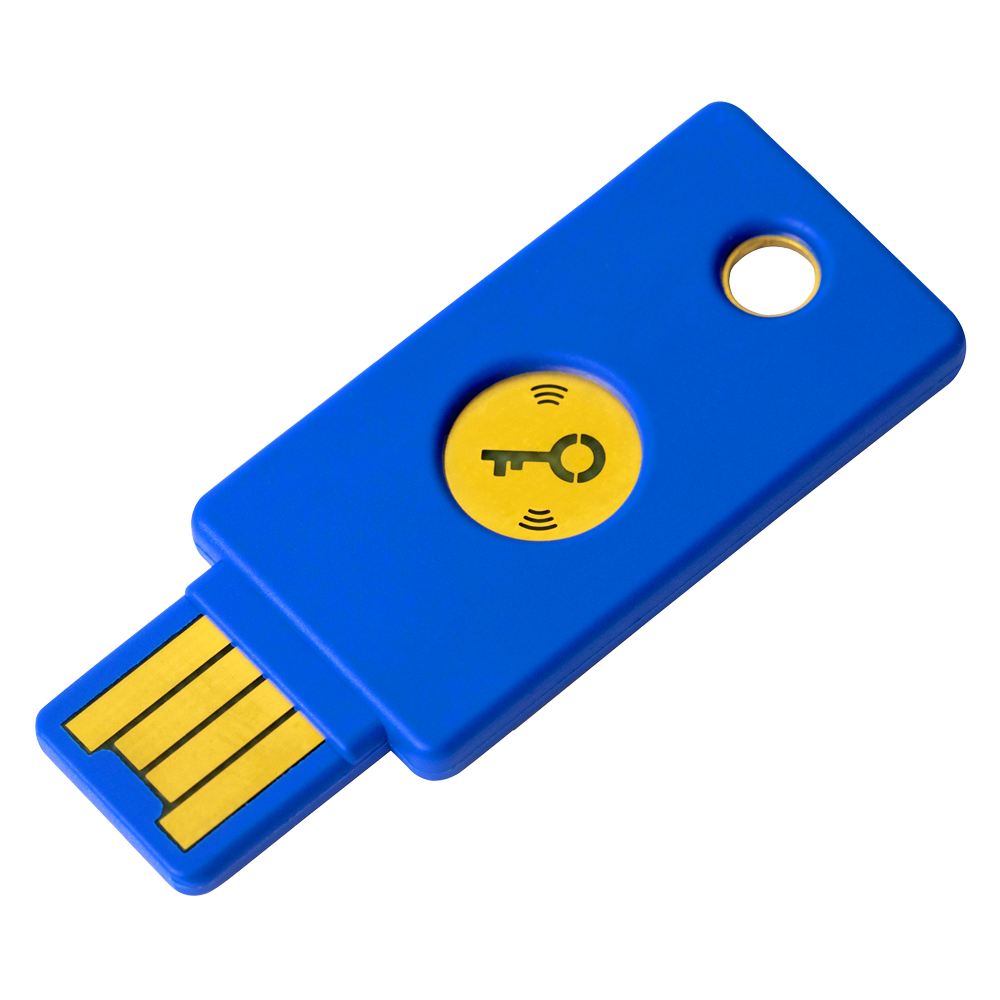
\includegraphics[width=0.4\linewidth]{resources/yubikey.png}
      \caption{The Security Key NFC, with the USB Interface and the Capacitive Touch Sensor on top of the key.}
      \label{fig:key}
\end{figure}

The YubiKey is composed by an USB Interface and a Capacitive Touch Sensor (Fig. \ref{fig:key}), useful for the Test of User Presence (TUP), which I will cover later.

The key supports to phases of the protocol: \emph{register}, which is useful to register the key to new websites and, in turn, register the website as trustworthy in the security key, and \emph{authenticate}, which lets the user authenticate into the website using the security key previously registered.

\subsection{Registration Protocol}\label{registration-protocol}
At the beginning of the registration, the user asks the website to add their new security key. The website (See Fig. \ref{fig:registration-protocol}) sends to the Client a challenge, which is a long enough random number generated to avoid man-in-the-middle attacks (the Client in this case is the Browser used by the user to authenticate).

\begin{figure}[h]
    \centering
    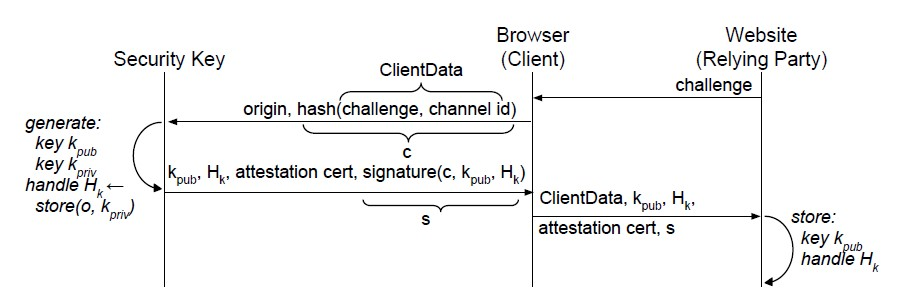
\includegraphics[width=\linewidth]{resources/registration-protocol.jpg}
    \caption{Security Key registration}
    \label{fig:registration-protocol}
\end{figure}

The Client, in turn, extracts the web origin (the website url) and hashes the ClientData. For the purpose of my sample web application, I will not cover the ClientData, but you can find more information at \citet{lang2016security}. I also used their illustrations for the message exchange of the registration and authentication protocols.

The web origin and the ClientData are then sent to the security key by the Client, and the security key generates a pair of asymmetric keys, plus the key Handle $H_k$. I will cover later the key Handle. As for now, assume that the security key stores the web origin and the private key for future use.

The security key then returns to the Client the public key, the key Handle and an attestation certificate, with in addition a signature over: 1. the hash sent previously by the Client, 2. the public key, 3. the key Handle, and 4. the web origin.

The Client simply forwards those information to the website, which will be able to verify the signature with the public key and verify wth the attestation certificate if the key is actually trustworthy.

\subsection{Authentication Protocol}\label{authentication-protocol}
The authentication protocol is very similar to the registration. See Fig.~\ref{fig:authentication-protocol} for details.

\begin{figure}[h]
    \centering
    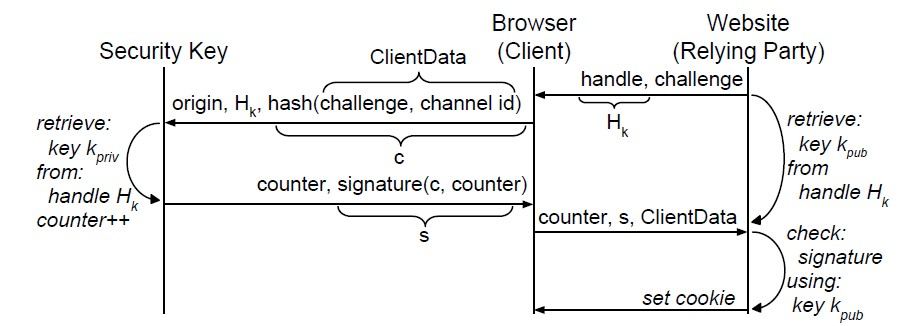
\includegraphics[width=\linewidth]{resources/authentication-protocol.jpg}
      \caption{Security Key authentication}
      \label{fig:authentication-protocol}
\end{figure}

When the user requests for authenticating, they will usually be prompted with a username-password interface, and afterwards a security key as second factor will be asked.

At this point, the website will send the challenge and the key Handle previously stored in the database. The Client will forward the same information of the registration along with the key Handle to the security key

Now the security key will use the private key for generating the signature, and the web origin associated to that private key to check if the website requesting the authentication is trustworthy, thus avoiding real-time phishing attacks, as I mentioned in Sec. \ref{introduction} \cite{reailton2015phishing}. The security key will return to the Client the signature and a counter, which is always incrementing and is used for avoiding cloning attacks. I will explain all these advantages more in detail in Sec. \ref{advantages}.

The Client will forwards the aforementioned information to the website, which will in turn verify if the security key is valid. In case the website finds out the key has been cloned, it invalidates it forever.

\subsection{Store and Retrieve Operations}\label{key-handle}
Those security keys are small embedded systems which only provides cryptographic measures for generating keys and computing encryption and decryption. This is why they are designed to avoid storing information. When I wrote in Sec. \ref{registration-protocol} to assume that the security key stores the private key and the web origin associated with it, it was a simplification. If the key stored all the websites used for authenticating, there would be to problems:
\begin{enumerate}
    \item The user would lose privacy, as their security key could be used to track their habits. In fact, habits information can be extracted by looking at which are the websites usually used by the user.
    \item The user should constantly check if the security key has run out of memory. Moreover, considering the embedded nature of the device, those technologies usually do not have much memory inside it. This would be a huge usability issue.
\end{enumerate}

To avoid those problems, the device leaves the website the job of storing information, harnessing a key Handle generated in registration phase. The key has two private keys that are never disclosed and that are not used for asymmetric cryptography. Those keys are used for generating the key Handle, which therefore the website cannot extract information from.

\begin{algorithm}[h]
    \caption{Store function}\label{alg:store}
    \begin{algorithmic}
    \Function{\textsc{store}}{$k_{priv}$, $o$}
        \State $o' \gets Encrypt(o)_{k_o}$
        \State $plaintext \gets Interleave(k_{priv}, o')$
        \State $H_k \gets Encrypt(plaintext)_{k_{wrap}}$
        \State \Return $H_k$
    \EndFunction
    \end{algorithmic}
\end{algorithm}

The \textsc{store} (See Alg. \ref{alg:store}) function takes as inputs the private key $k_{priv}$ just generated during the registration phase, and the web origin $o$. It encrypts the web origin using one of the two keys never disclosed (which we will call $k_o$) and then interleaves $k_{priv}$ with the origin encrypted. The resulting string is encrypted again with the second key (called $k_{wrap}$), generating the key Handle $H_k$.

The \textsc{retrieve} function will take as inputs the web origin $o$ and the key Handle $H_k$ previously stored by the website. Similarly to the \textsc{store} function, it uses $k_o$ and $K_{wrap}$ to encrypt and decrypt where necessary. More details are shown at Alg. \ref{alg:retrieve}

\begin{algorithm}[h]
    \caption{Retrieve function}\label{alg:retrieve}
    \begin{algorithmic}
    \Function{\textsc{retrieve}}{$H_k$, $o$}
        \State $o' \gets Encrypt(o)_{k_o}$
        \State $(K_{priv}, o'') \gets Denterleave(plaintext)$
        \State $\textsc{constant-time check(o' == o'')}$
        \State \Return $k_{priv}$
    \EndFunction
    \end{algorithmic}
\end{algorithm}

I would like to have the reader focused on the advantages behind generating the $H_k$. Being encrypted with never disclosed keys, the website cannot retrieve any information from the key Handle, hence the user privacy is ensured. In addition, the key Handle associates each private key to the correspondent web origin. Therefore, during the authentication, the device is able to compare the website's web origin with the web origin associated to the private key. If the URKs appear different, the device recognizes a potential real-time phishing attack and drops the authentication. In this way the key is able to ``store'' potentially an infinite amount of websites.

\subsection{Security Key Advantages}\label{advantages}
There are several advantages behind using a Security Key over other OTPs technologies, such as smartphones or messages, and I outlined them in Sec. \ref{related-work}. Now, after outlining the protocol, I would like to explain how the messages exchanged denote those advantages \cite{lang2016security}:
\begin{itemize}
    \item \textbf{\textsc{challenge}:} This information is a random number used in many protocols to avoid man-in-the-middle attacks. It is actually a standard method for any protocol in the web, but it is worth to mention.
    \item \textbf{Key Handle:} As I explained in Sec. \ref{key-handle}, the Key Handle gives the user more privacy because the websites cannot be tracked on the device, and in addition solves the problem of having a limited amount of memory.
    \item \textbf{Attestation Certificate:} To let the websites know that the security key is a device trustworthy and that it reflects the FIDO2 and U2F protocol, there must be some check on the validity of the hardware. However, a unique identifier would be too privacy intrusive for the user. To solve this issue, the attestation certificate of the security key is released with batches. In this way, a subset of devices is identified with each attestation certificate and the user cannot be tracked, unless they are the only ones who bought that precise batch.
    \item \textbf{\textsc{counter}:} The device has an internal counter that gets incremented each time the user authenticates into a website. The counter is supposed to be always incremental, so that if the key gets cloned, the website can detect a decrement of it and, if so, invalidate that security key.
    \item \textbf{Test of User Presence (TUP):} Each device has a sensor that can detect if the user is present in the moment they are authenticating. The device I used \ref{fig:key} has a capacitive sensor on the top, and other keys have even a fingerprint scanner\footnote{\url{https://www.yubico.com/products/yubikey-bio-series/}}. In those cases, the ``to have'' and ``to be'' factors are combined together.
\end{itemize}